% Created by tikzDevice version 0.12.3.1 on 2021-12-15 13:58:10
% !TEX encoding = UTF-8 Unicode
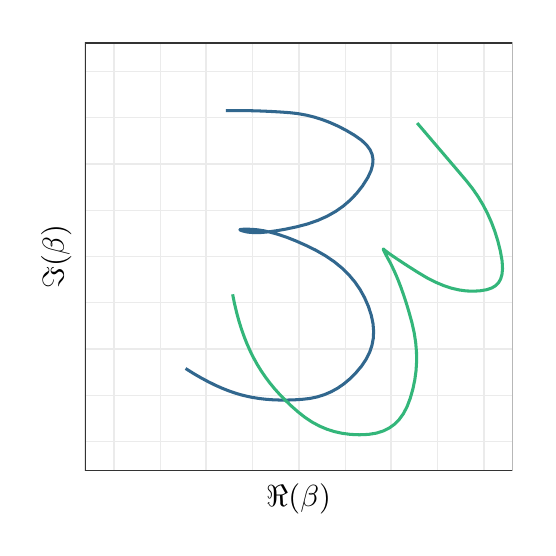
\begin{tikzpicture}[x=1pt,y=1pt]
\definecolor{fillColor}{RGB}{255,255,255}
\path[use as bounding box,fill=fillColor,fill opacity=0.00] (0,0) rectangle (180.67,180.67);
\begin{scope}
\path[clip] (  0.00,  0.00) rectangle (180.67,180.67);
\definecolor{drawColor}{RGB}{255,255,255}
\definecolor{fillColor}{RGB}{255,255,255}

\path[draw=drawColor,line width= 0.6pt,line join=round,line cap=round,fill=fillColor] (  0.00,  0.00) rectangle (180.67,180.68);
\end{scope}
\begin{scope}
\path[clip] ( 20.71, 20.71) rectangle (175.17,175.17);
\definecolor{fillColor}{RGB}{255,255,255}

\path[fill=fillColor] ( 20.71, 20.71) rectangle (175.17,175.17);
\definecolor{drawColor}{gray}{0.92}

\path[draw=drawColor,line width= 0.3pt,line join=round] ( 20.71, 47.80) --
	(175.17, 47.80);

\path[draw=drawColor,line width= 0.3pt,line join=round] ( 20.71, 81.23) --
	(175.17, 81.23);

\path[draw=drawColor,line width= 0.3pt,line join=round] ( 20.71,114.66) --
	(175.17,114.66);

\path[draw=drawColor,line width= 0.3pt,line join=round] ( 20.71,148.09) --
	(175.17,148.09);

\path[draw=drawColor,line width= 0.3pt,line join=round] ( 47.80, 20.71) --
	( 47.80,175.17);

\path[draw=drawColor,line width= 0.3pt,line join=round] ( 81.23, 20.71) --
	( 81.23,175.17);

\path[draw=drawColor,line width= 0.3pt,line join=round] (114.66, 20.71) --
	(114.66,175.17);

\path[draw=drawColor,line width= 0.3pt,line join=round] (148.09, 20.71) --
	(148.09,175.17);

\path[draw=drawColor,line width= 0.6pt,line join=round] ( 20.71, 31.08) --
	(175.17, 31.08);

\path[draw=drawColor,line width= 0.6pt,line join=round] ( 20.71, 64.51) --
	(175.17, 64.51);

\path[draw=drawColor,line width= 0.6pt,line join=round] ( 20.71, 97.94) --
	(175.17, 97.94);

\path[draw=drawColor,line width= 0.6pt,line join=round] ( 20.71,131.38) --
	(175.17,131.38);

\path[draw=drawColor,line width= 0.6pt,line join=round] ( 20.71,164.81) --
	(175.17,164.81);

\path[draw=drawColor,line width= 0.6pt,line join=round] ( 31.08, 20.71) --
	( 31.08,175.17);

\path[draw=drawColor,line width= 0.6pt,line join=round] ( 64.51, 20.71) --
	( 64.51,175.17);

\path[draw=drawColor,line width= 0.6pt,line join=round] ( 97.94, 20.71) --
	( 97.94,175.17);

\path[draw=drawColor,line width= 0.6pt,line join=round] (131.38, 20.71) --
	(131.38,175.17);

\path[draw=drawColor,line width= 0.6pt,line join=round] (164.81, 20.71) --
	(164.81,175.17);
\definecolor{drawColor}{RGB}{49,103,142}

\path[draw=drawColor,line width= 1.1pt,line join=round] ( 57.06, 57.51) --
	( 59.89, 55.73) --
	( 62.61, 54.15) --
	( 65.24, 52.74) --
	( 67.77, 51.49) --
	( 70.20, 50.41) --
	( 72.56, 49.47) --
	( 74.83, 48.68) --
	( 77.02, 48.02) --
	( 79.15, 47.49) --
	( 81.31, 47.05) --
	( 83.55, 46.69) --
	( 85.88, 46.41) --
	( 88.31, 46.22) --
	( 90.84, 46.12) --
	( 93.48, 46.10) --
	( 96.23, 46.18) --
	( 99.10, 46.36) --
	(101.98, 46.69) --
	(104.68, 47.26) --
	(107.24, 48.07) --
	(109.67, 49.11) --
	(112.01, 50.40) --
	(114.27, 51.96) --
	(116.47, 53.81) --
	(118.62, 55.98) --
	(120.74, 58.50) --
	(122.37, 60.97) --
	(123.58, 63.42) --
	(124.41, 65.87) --
	(124.88, 68.38) --
	(125.01, 71.00) --
	(124.78, 73.77) --
	(124.16, 76.74) --
	(123.11, 79.97) --
	(121.73, 83.12) --
	(120.11, 86.05) --
	(118.23, 88.79) --
	(116.07, 91.35) --
	(113.62, 93.77) --
	(110.83, 96.05) --
	(107.68, 98.21) --
	(104.12,100.25) --
	(100.36,102.09) --
	( 96.88,103.63) --
	( 93.67,104.90) --
	( 90.70,105.91) --
	( 87.97,106.68) --
	( 85.45,107.25) --
	( 83.14,107.62) --
	( 81.00,107.81) --
	( 79.03,107.84) --
	( 77.77,107.82) --
	( 77.07,107.77) --
	( 76.77,107.71) --
	( 76.69,107.67) --
	( 76.69,107.64) --
	( 76.81,107.56) --
	( 77.19,107.40) --
	( 78.01,107.13) --
	( 79.15,106.86) --
	( 80.57,106.68) --
	( 82.30,106.61) --
	( 84.38,106.66) --
	( 86.85,106.87) --
	( 89.76,107.26) --
	( 93.14,107.85) --
	( 97.03,108.67) --
	(101.15,109.74) --
	(104.87,111.04) --
	(108.23,112.55) --
	(111.28,114.27) --
	(114.05,116.21) --
	(116.57,118.38) --
	(118.87,120.79) --
	(120.98,123.47) --
	(122.89,126.47) --
	(124.07,129.01) --
	(124.66,131.19) --
	(124.78,133.09) --
	(124.47,134.84) --
	(123.74,136.52) --
	(122.51,138.21) --
	(120.66,139.98) --
	(118.01,141.84) --
	(115.08,143.57) --
	(112.18,145.08) --
	(109.29,146.37) --
	(106.42,147.46) --
	(103.54,148.36) --
	(100.66,149.07) --
	( 97.75,149.60) --
	( 94.81,149.94) --
	( 91.85,150.16) --
	( 88.91,150.34) --
	( 85.98,150.48) --
	( 83.07,150.60) --
	( 80.19,150.67) --
	( 77.31,150.72) --
	( 74.46,150.73) --
	( 71.62,150.71) --
	( 71.62,150.71);
\definecolor{drawColor}{RGB}{51,182,122}

\path[draw=drawColor,line width= 1.1pt,line join=round] ( 74.06, 84.33) --
	( 74.74, 80.94) --
	( 75.51, 77.70) --
	( 76.35, 74.62) --
	( 77.27, 71.69) --
	( 78.27, 68.89) --
	( 79.33, 66.23) --
	( 80.47, 63.69) --
	( 81.68, 61.27) --
	( 82.96, 58.96) --
	( 84.34, 56.72) --
	( 85.85, 54.50) --
	( 87.49, 52.31) --
	( 89.26, 50.15) --
	( 91.17, 48.02) --
	( 93.24, 45.90) --
	( 95.45, 43.80) --
	( 97.84, 41.71) --
	(100.34, 39.75) --
	(102.88, 38.09) --
	(105.46, 36.70) --
	(108.11, 35.58) --
	(110.85, 34.71) --
	(113.70, 34.08) --
	(116.69, 33.70) --
	(119.84, 33.56) --
	(123.18, 33.70) --
	(126.04, 34.17) --
	(128.50, 34.94) --
	(130.64, 36.00) --
	(132.52, 37.35) --
	(134.21, 39.04) --
	(135.72, 41.12) --
	(137.07, 43.67) --
	(138.25, 46.78) --
	(139.19, 50.08) --
	(139.88, 53.38) --
	(140.33, 56.69) --
	(140.54, 60.03) --
	(140.50, 63.42) --
	(140.21, 66.87) --
	(139.67, 70.40) --
	(138.86, 74.04) --
	(137.86, 77.65) --
	(136.86, 81.00) --
	(135.85, 84.08) --
	(134.84, 86.92) --
	(133.84, 89.53) --
	(132.83, 91.91) --
	(131.83, 94.07) --
	(130.84, 96.04) --
	(129.86, 97.83) --
	(129.19, 99.08) --
	(128.79, 99.90) --
	(128.58,100.37) --
	(128.50,100.60) --
	(128.49,100.67) --
	(128.50,100.68) --
	(128.57,100.65) --
	(128.75,100.49) --
	(129.10,100.19) --
	(129.68, 99.74) --
	(130.53, 99.12) --
	(131.70, 98.29) --
	(133.27, 97.23) --
	(135.26, 95.91) --
	(137.75, 94.30) --
	(140.79, 92.37) --
	(144.15, 90.35) --
	(147.32, 88.73) --
	(150.31, 87.47) --
	(153.15, 86.53) --
	(155.87, 85.90) --
	(158.47, 85.54) --
	(160.99, 85.44) --
	(163.46, 85.59) --
	(165.90, 85.99) --
	(167.74, 86.63) --
	(169.11, 87.46) --
	(170.13, 88.50) --
	(170.88, 89.79) --
	(171.38, 91.44) --
	(171.59, 93.58) --
	(171.44, 96.34) --
	(170.82, 99.86) --
	(169.91,103.53) --
	(168.82,107.03) --
	(167.56,110.38) --
	(166.13,113.59) --
	(164.52,116.67) --
	(162.73,119.64) --
	(160.76,122.50) --
	(158.58,125.27) --
	(156.28,127.98) --
	(154.00,130.66) --
	(151.74,133.31) --
	(149.50,135.94) --
	(147.28,138.54) --
	(145.08,141.12) --
	(142.90,143.68) --
	(140.74,146.20) --
	(140.74,146.20);
\definecolor{drawColor}{gray}{0.20}

\path[draw=drawColor,line width= 0.6pt,line join=round,line cap=round] ( 20.71, 20.71) rectangle (175.17,175.17);
\end{scope}
\begin{scope}
\path[clip] (  0.00,  0.00) rectangle (180.67,180.67);
\definecolor{drawColor}{RGB}{0,0,0}

\node[text=drawColor,anchor=base,inner sep=0pt, outer sep=0pt, scale=  1.10] at ( 97.94,  7.64) {$\Re(\beta)$};
\end{scope}
\begin{scope}
\path[clip] (  0.00,  0.00) rectangle (180.67,180.67);
\definecolor{drawColor}{RGB}{0,0,0}

\node[text=drawColor,rotate= 90.00,anchor=base,inner sep=0pt, outer sep=0pt, scale=  1.10] at ( 13.08, 97.94) {$\Im(\beta)$};
\end{scope}
\end{tikzpicture}
